\documentclass{article}
\usepackage{tikz}
\usetikzlibrary{positioning}
\begin{document}
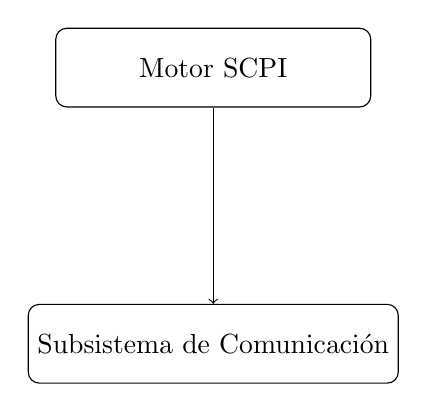
\begin{tikzpicture}[
    block/.style={draw, rectangle, rounded corners, minimum width=4cm, minimum height=1cm, align=center}
]
\node[block] (scpi) at (0,0) {Motor SCPI};
\node[block, below=1.5cm of scpi] (comm) at (0,-1.5) {Subsistema de Comunicación};
\draw[->] (scpi) -- (comm);
\end{tikzpicture}
\end{document}